\chapter{Auswertung}

\section{Dopplerverbreitertes Spektrum}

\begin{figure}[ht]
  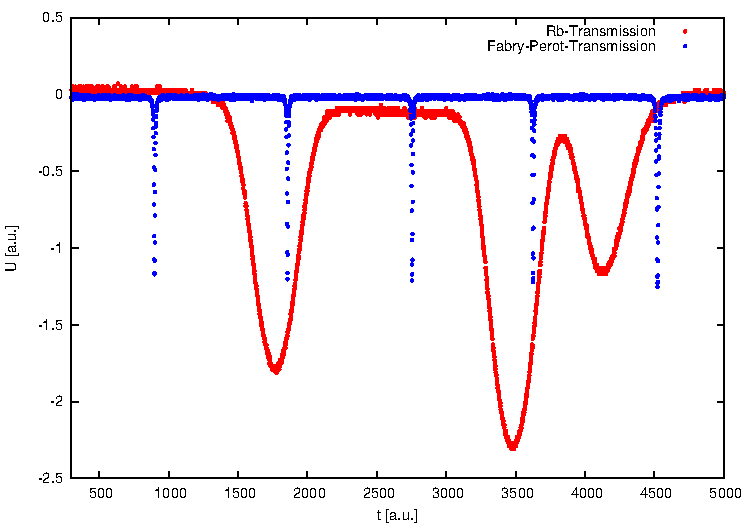
\includegraphics[width=0.9\textwidth]{./dopplerspektrum-messung.pdf}
  \caption{Die Spannung der differentiellen Photodiode (proportional zur Intensit�t
  		    des durch die Rb-Zelle transmittierten Lichts in willk�rlichen Einheiten)
			und entsprechend die Spannung hinter dem Fabry-P�rot-Resonator
		    aufgetragen gegen die Zeit $t$, w�hrend der der Frequenzbereich des Lasers 
			durchgefahren wird, ebenfalls in willk�rlichen Einheiten.}
\label{fig:dopplerroh}
\end{figure}

In Abbildung \ref{fig:dopplerroh} sind die vom Oszilloskop aufgenommenen Messdaten
dargestellt. Zu sehen sind von links nach rechts die 85F2-, 85F3- und 87F2-Resonanzen
(85F2 heisst hier z.B. die �berlagerung der drei �berg�nge vom $F=2$--Grundniveau des
$^{85}\text{Rb}$--Isotops)

Die Resonanzen des Fabry-P�rot-Signals entsprechen konstanten Frequenzabst�nden und dies
wird als Grundlage f�r einen Fit durch ein Polynom dritten Grades $f$ genutzt
(f�nf Messpunkte $(t_i,f(t_i))$ bei den Zeitpunkten $t_i$ der Resonanzen mit
gleichem $f(t)$-Abstand), siehe Abbildung \ref{fig:xumskalierung}.
\begin{figure}[!ht]
  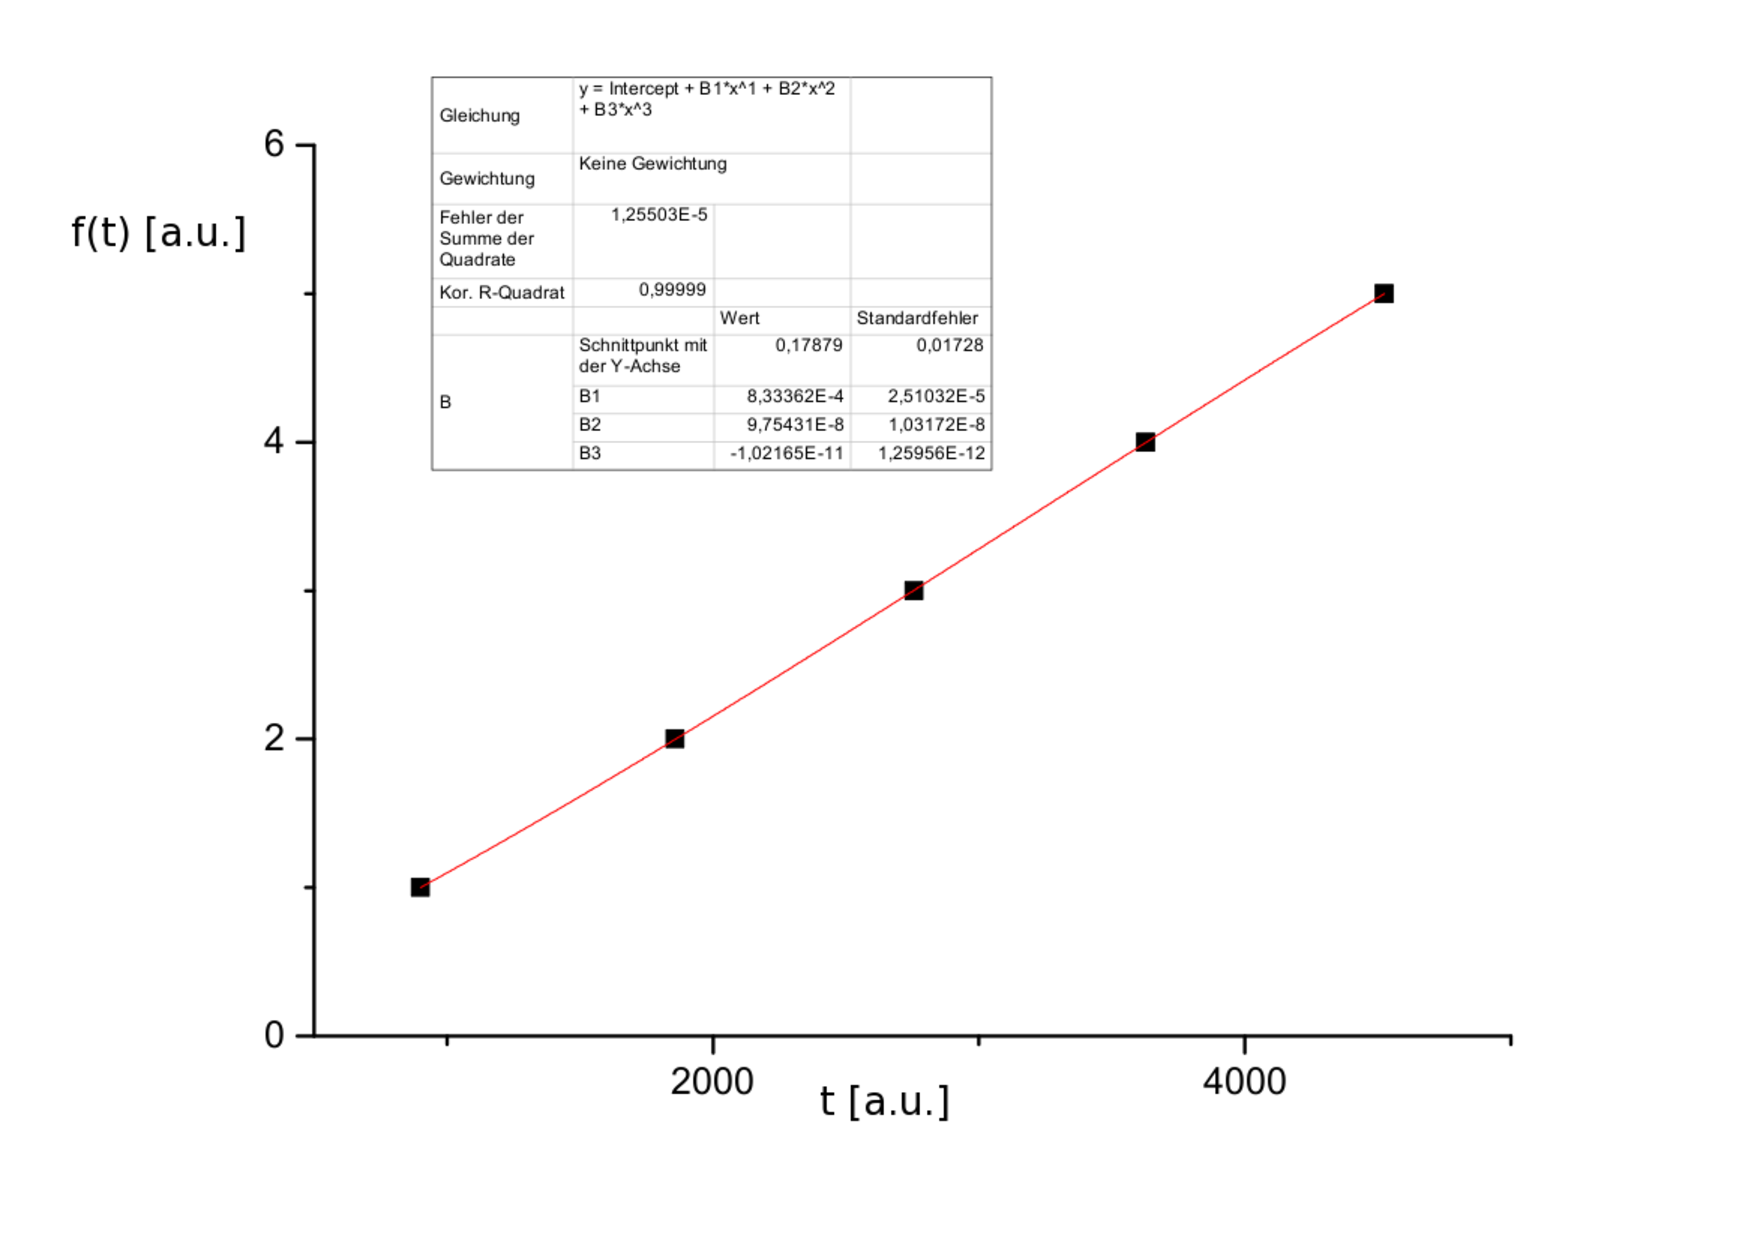
\includegraphics[width=1\textwidth]{./xumskalierung.pdf}
  \caption{Umskalierung der Messzeitachse zur Frequenzachse}
\label{fig:xumskalierung}
\end{figure}
Wenn dann das Dopplerspektrum $I$ gegen $f(t)$ aufgetragen wird, stimmt die Skalierung
bis auf eine lineare Umskalierung, die abschliessend durch Kenntnis der Position und
Abst�nde der Spektrallinien erfolgt. Vor dieser linearen Umskalierung werden die
$(I,f(t))$--Daten durch eine Summe von zwei �berlagerungen f�r die 85F2- und
85F3-Resonanzen
aus jeweils drei Gau�profilen
mit gleicher Breite (die nach \eqref{eq:gausstemp} der Temperatur des Rb-Gases entspricht)
und durch Literaturwerte [2] vorgegebene Amplitudenverh�ltnisse und einer beliebigen
Gau�funktion f�r die rechte 87F2-Resonanz gefittet (siehe Anhang A).

\begin{figure}[ht]
  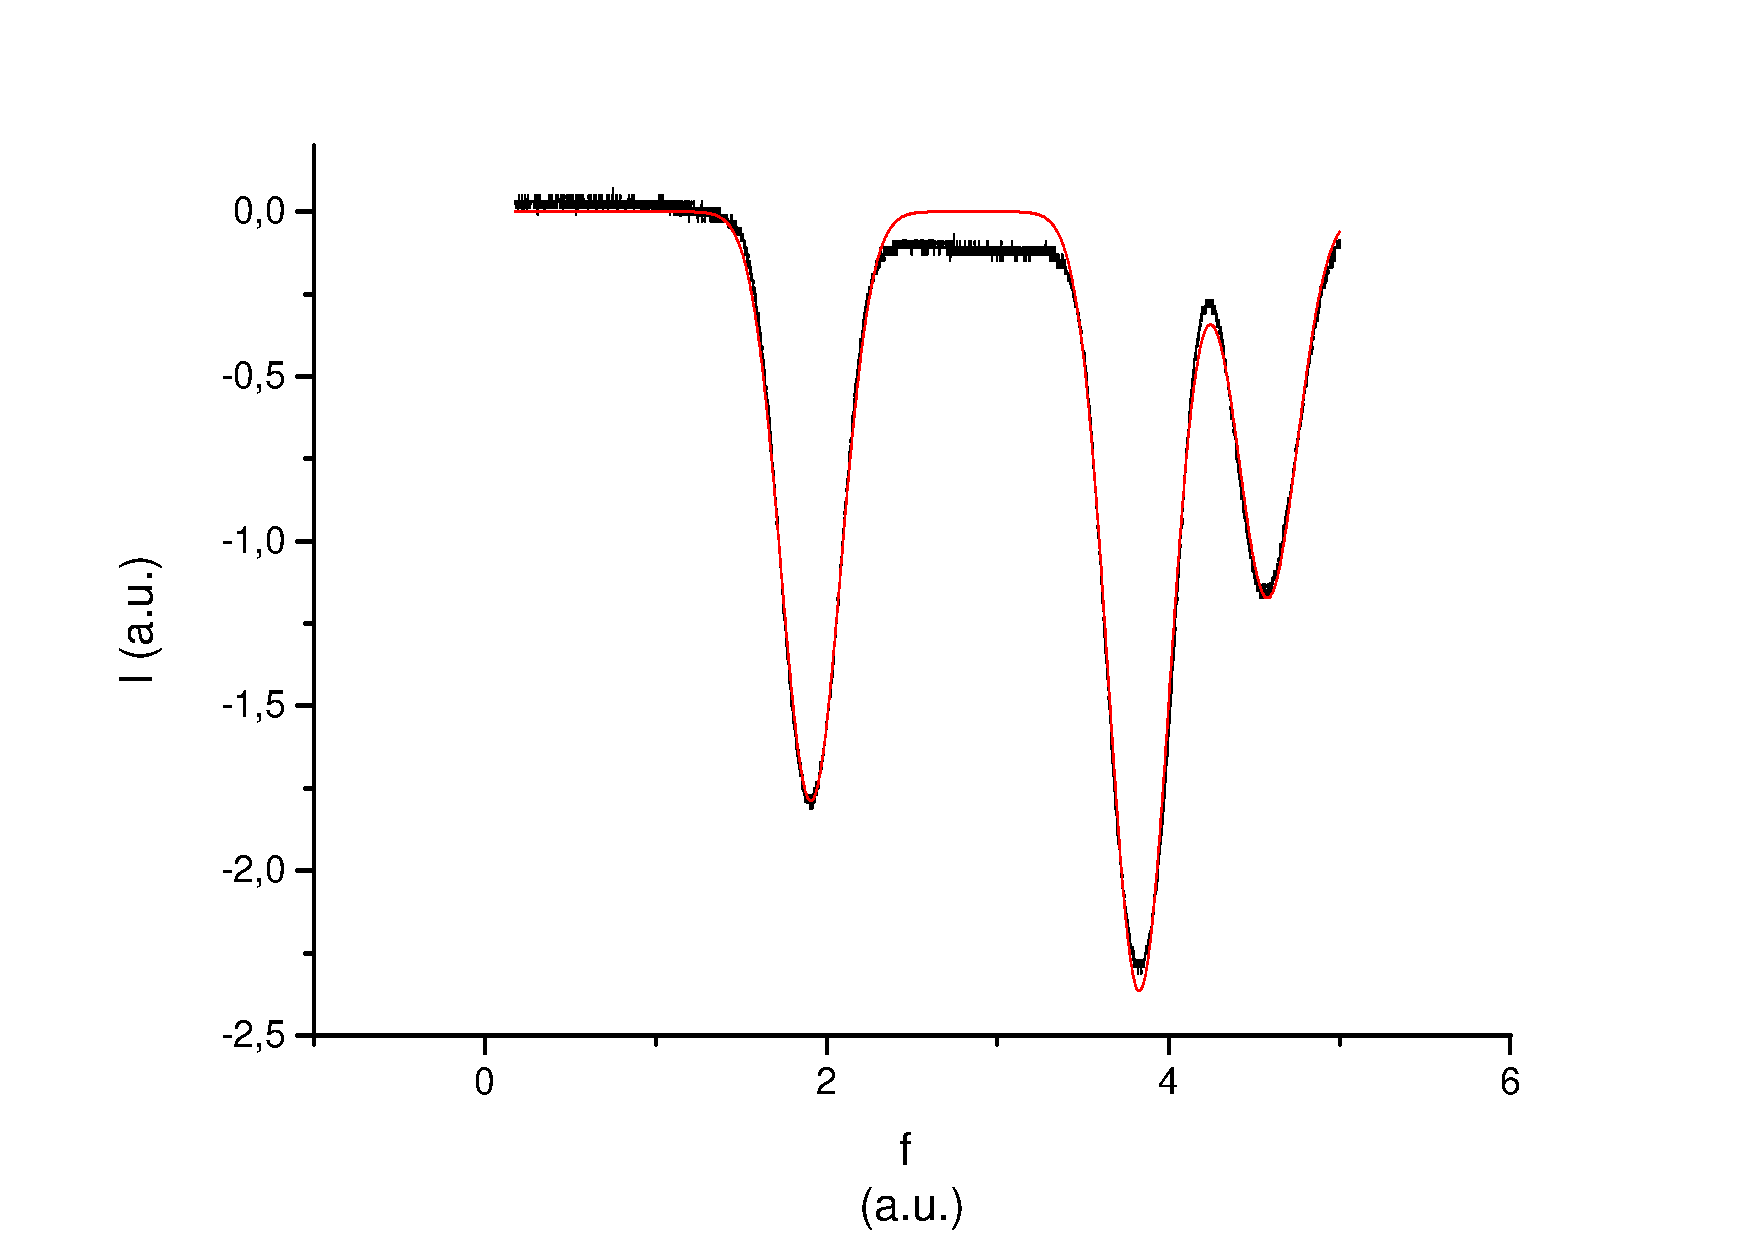
\includegraphics[width=1\textwidth]{./dopplerfit-plot.pdf}
  \caption{Gemessenes Dopplerspektrum in willk�rlichen Einheiten gegen die
  		umskalierte $f(t)$--Achse in Schwarz; Fit in Rot}
\label{fig:dopplerfit}
\end{figure}

Aus dem Fit ergibt sich eine gemeinsame halbe $\frac{1}{e}$--Breite $w$ der �berlagerten
Gau�profile f�r die 85F2- und 85F3-Resonanzen in Einheiten der $f(t)$--Achse als Parameter
des Fits, aus der
wir die volle Halbwertsbreite in MHz durch Umrechnung der Breitenarten
(halbe $\frac{1}{e}$--Breite in volle Halbwertsbreite) und
Skalierung erhalten, da die wahren relativen
Abst�nde der Resonanzen aus der Literatur [2] bekannt sind.

Wir erhalten somit:
\begin{equation}
	w = (406,5 \pm 0,8) \text{ MHz} \nonumber
\end{equation}

Mit Gleichung \eqref{eq:gausstemp} ergibt sich daraus f�r die Temperatur des Rb-Gases
\begin{equation}
	T = (432,1 \pm 1,7) \text{ K} \nonumber
\end{equation}



\section{Dopplerfreie S�ttigungsspektroskopie}

\subsection{Messung der Strahltaille}

In Abbildung \ref{fig:strahlbreite} sind die Messergebnisse der Leistungen $P_x$ und $P_y$
des durchgelassenen
Laserstrahls bei teilweiser Abdeckung durch die Rasierklinge mit Positionen $x$ aus
horizontaler Richtung bzw. $y$ aus vertikaler Richtung dargestellt. Die Nullpunkte
von $x$ und $y$ sind beliebig und irrelevant f�r die Auswertung.

Ebenfalls in Abbildung \ref{fig:strahlbreite} zu sehen sind die Fits der Messpunkte mit
Fehlerfunktionen nach \eqref{eq:yerrfct} und \eqref{eq:xerrfct}.

Aus den Fits ergeben sich die halben $\frac{1}{e^2}$--Breiten $w_x$ und $w_y$ der
als transversal gau�f�rmig verteilt angenommenen Intensit�t des Laserstrahls:

\begin{equation}
	\begin{split}
	w_x &= (1,60 \pm 0,09) \text{ mm} \\
	w_y &= (1,51 \pm 0,014) \text{ mm}
	\end{split} \nonumber
\end{equation}

\begin{figure}[!h]
  \subfigure[Strahlabdeckung aus horizontaler Richtung $x$]{
  	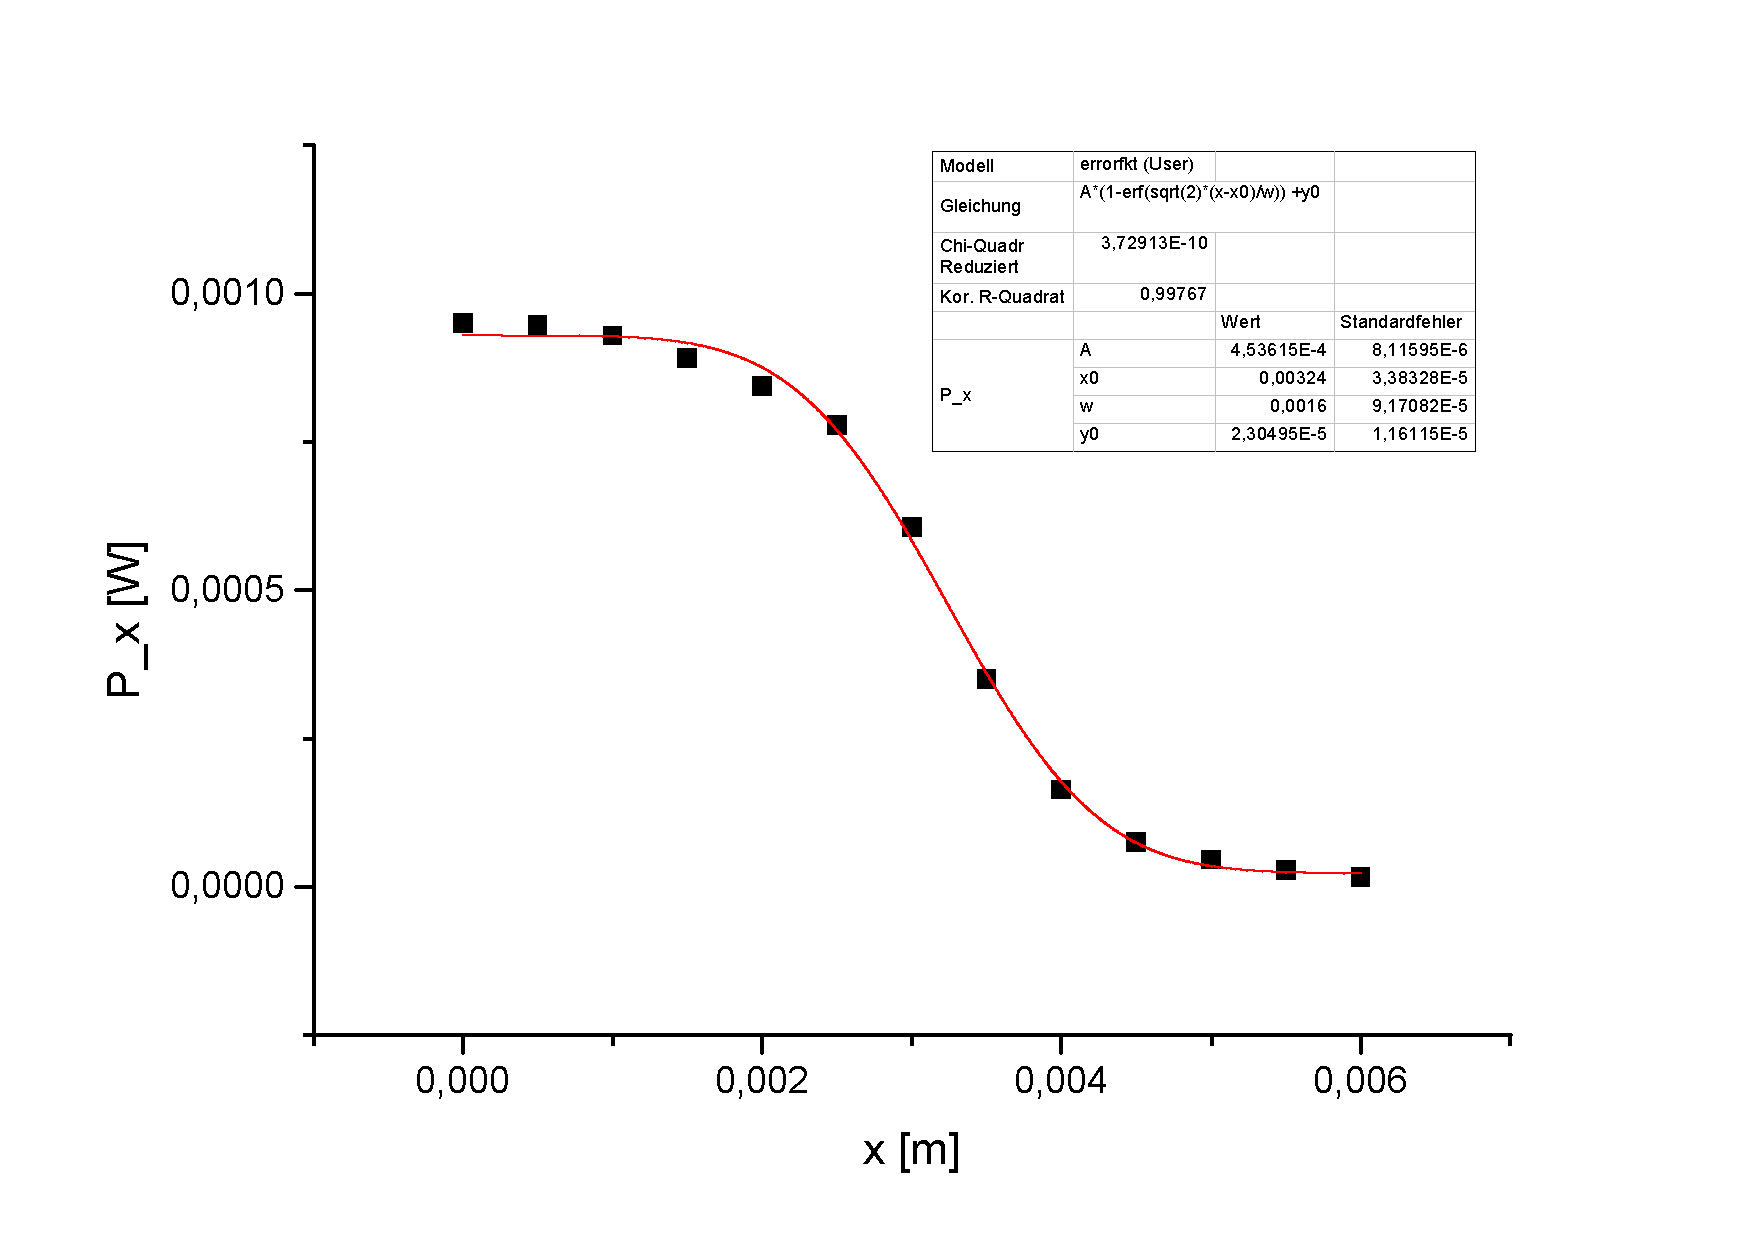
\includegraphics[width=1\textwidth]{./xstrahlbreite.pdf}
  }
  \subfigure[Strahlabdeckung aus horizontaler Richtung $y$]{
  	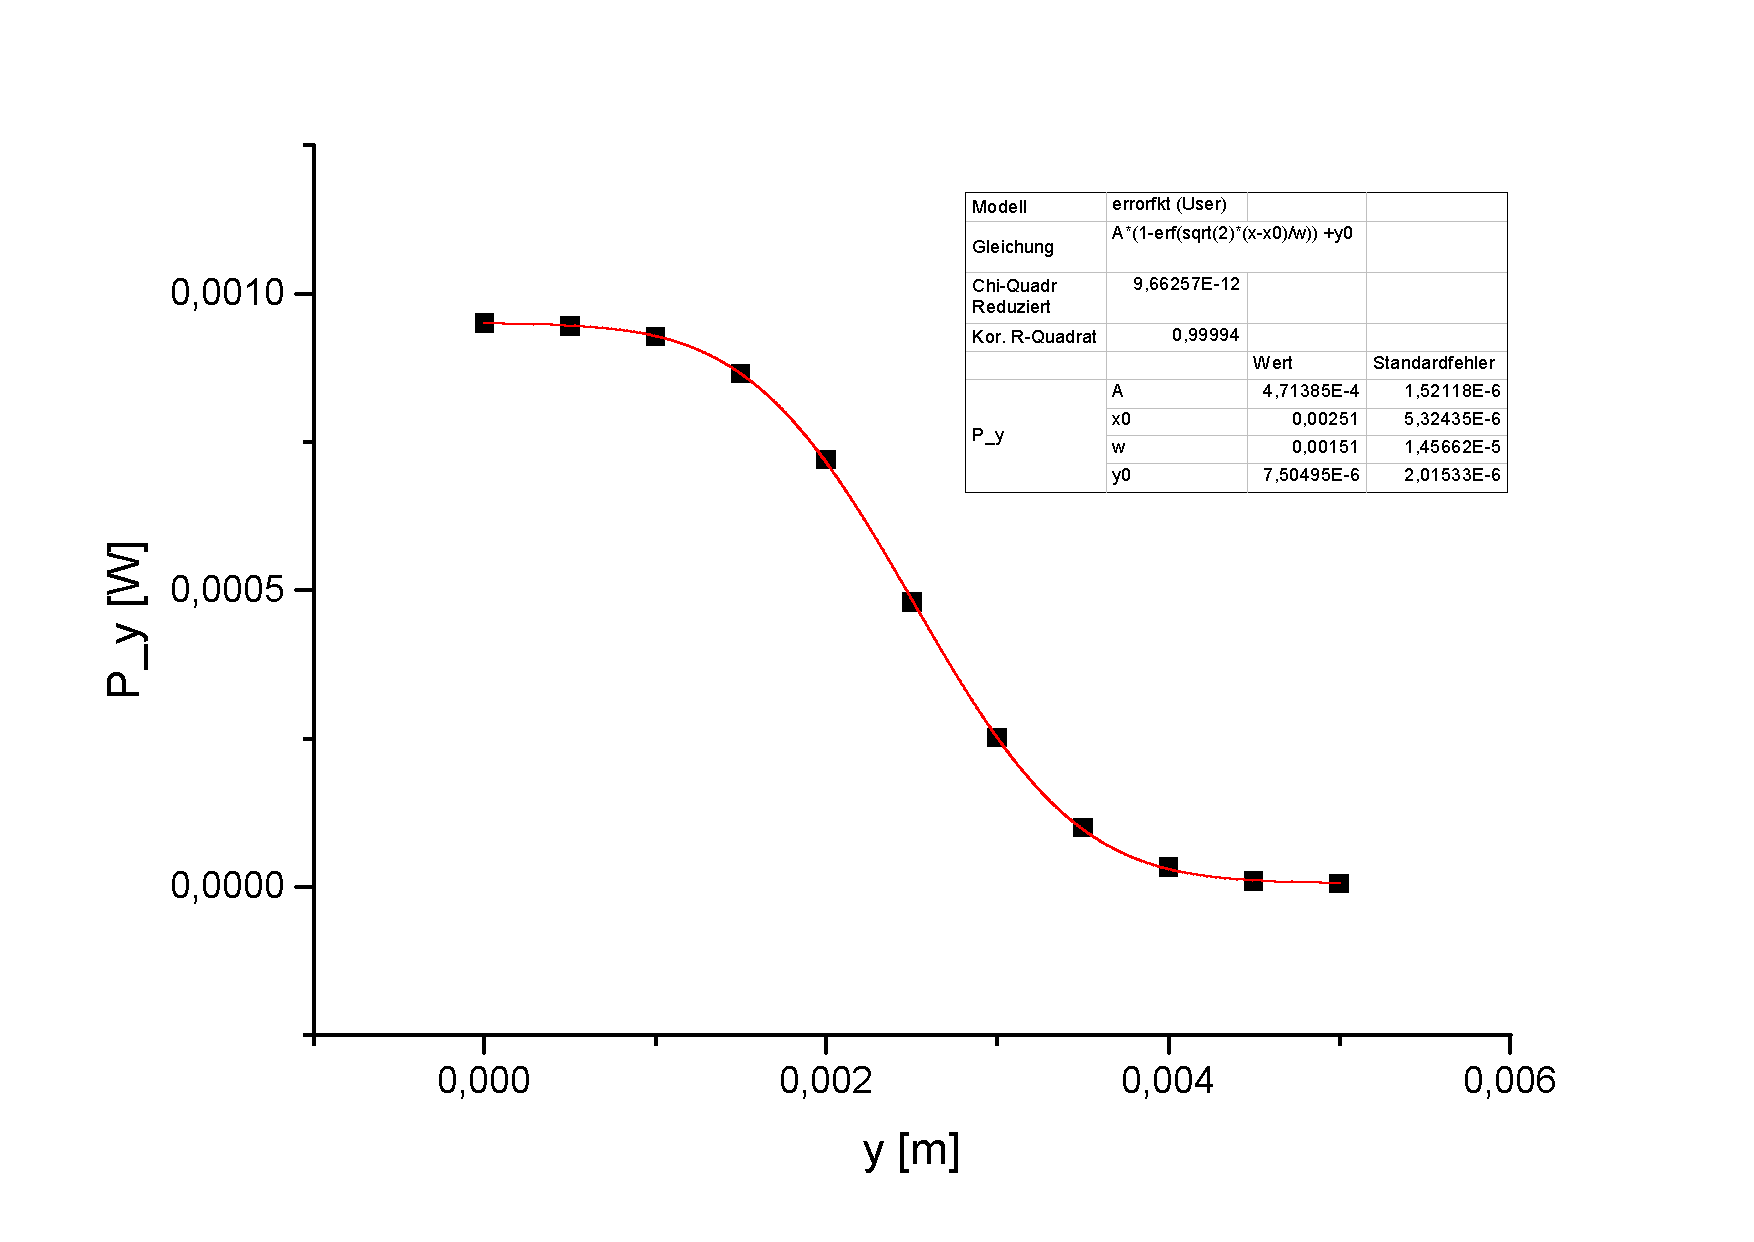
\includegraphics[width=1\textwidth]{./ystrahlbreite.pdf}
  }
  \caption{Messung der durchgelassenen Leistung bei Abdeckung durch eine Rasierklinge
  	  			in Schwarz; Fit mit Fehlerfunktion in Rot}
\label{fig:strahlbreite}
\end{figure}
\clearpage
\subsection{Bestimmung der nat�rlichen Linienbreite und S�ttigungsintensit�t}

Mithilfe der oben bestimmten Strahlbreiten $w_x$ und $w_y$ und Gleichung
\eqref{eq:intensitaet} k�nnen wir den verschiedenen Leistungen des Pumpstrahls,
zu denen wir jeweils das 87F2-Spektrum aufgenommen haben, die entsprechenden
Pumpstrahl-Intensit�ten zuordnen.
Jedes zu den verschiedenen Intensit�ten aufgenommene Spektrum wird mit
einer Summe von sechs Lorentzprofilen mit gleichen Halbwertsbreiten f�r
die drei Energie�berg�nge und die drei Crossover-Resonanzen, einer
Gau�-Funktion zur N�herung des Signaluntergrunds und einer konstanten Verschiebung gefittet
(siehe Anhang A).
Dabei sind die Verh�ltnisse
der Abst�nde der sechs Resonanzen aus der Literatur [2] und Theorie bekannt.
In Abbildung \ref{fig:400mukrow} ist beispielhaft die Messung bei der
Pumpstrahlleistung 400 $\mu$W zusammen mit dem Fitergebnis dargestellt.

\begin{figure}[!h]
  	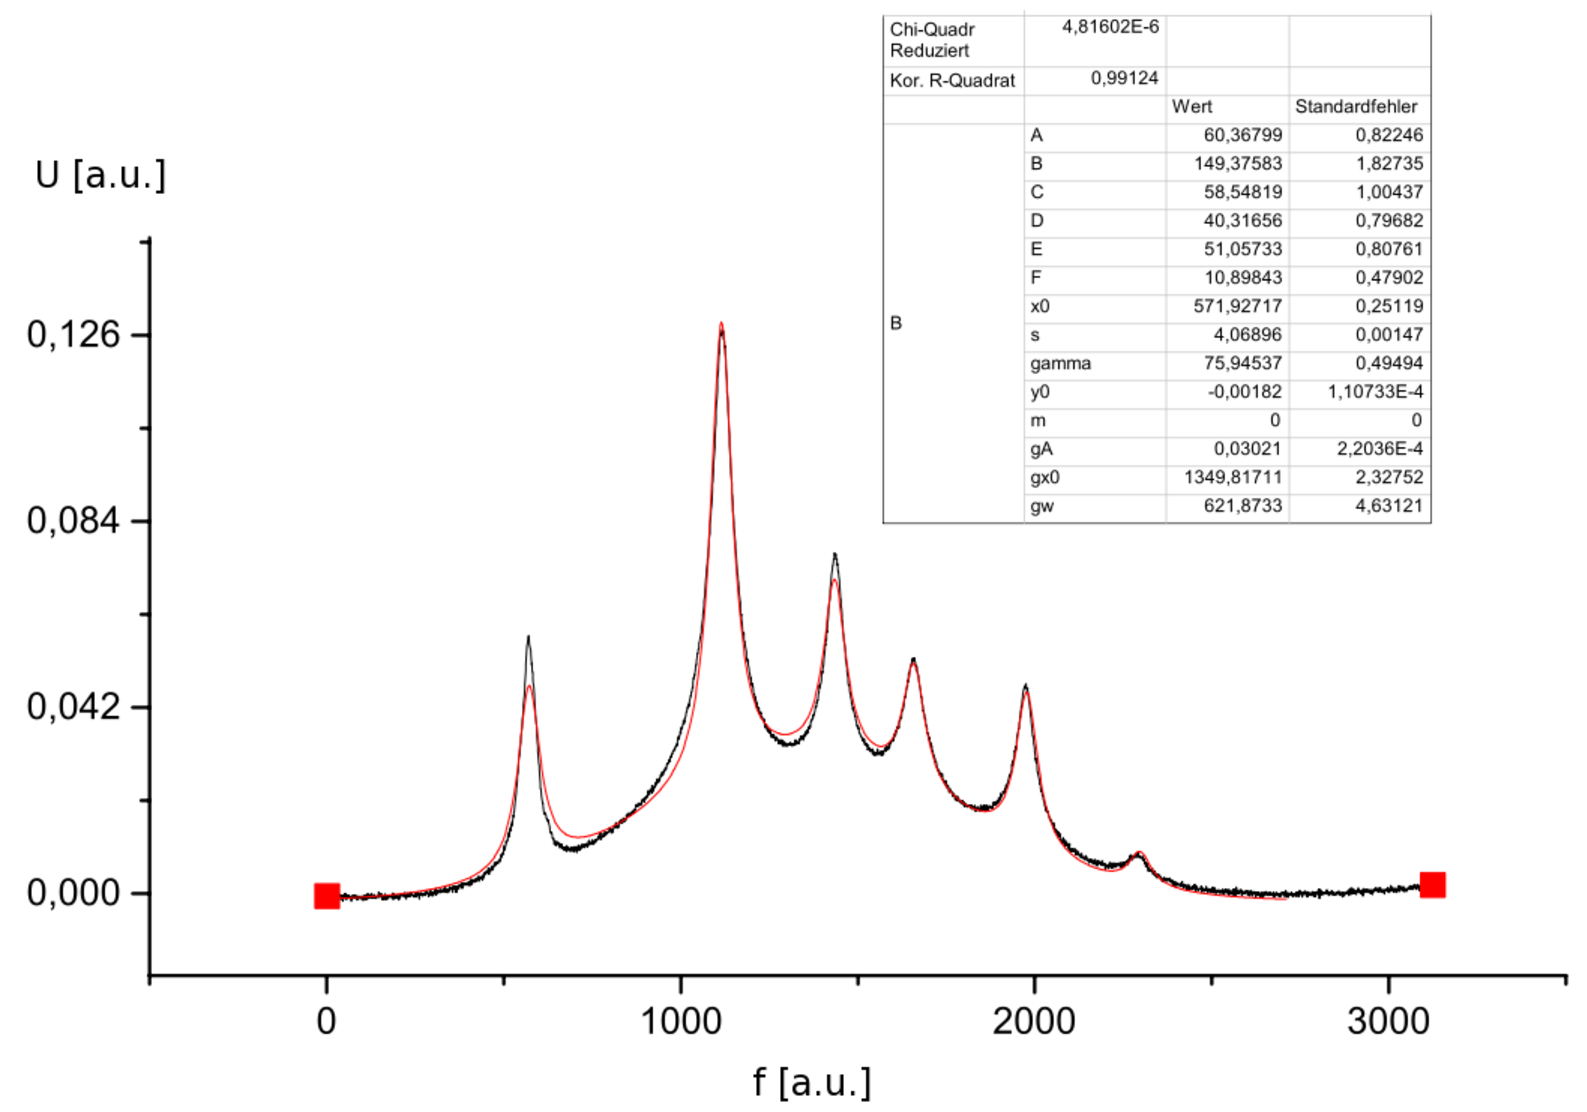
\includegraphics[width=1\textwidth]{./400uW.pdf}
  \caption{Messung der Aufspaltung der 87F2-Linie bei Pumpstrahlleistung 400 $\mu$W}
\label{fig:400mukrow}
\end{figure}

Wir erhalten also zu jeder Leistung $P$ des Pumpstrahls durch den Fit des
entsprechenden Spektrums als Parameter die volle
Halbwertsbreite $\Gamma$ der leistungsverbreiterten Resonanzen, die nach Gleichung
\eqref{eq:mitformel} von $I$ abh�ngt, welches wiederum nach \eqref{eq:intensitaet} von
$P$ abh�ngt. Durch einen Fit der Messwertepaare $(P,\Gamma)$
mit dem theoretischen Verlauf nach \eqref{eq:mitformel} und \eqref{eq:intensitaet}
werden dann die nat�rliche
Linienbreite $\gamma$ und die S�ttigungsintensit�t $I_{\text{sat}}$ von Rubidium bestimmt.
\clearpage

\begin{figure}[!h]
  	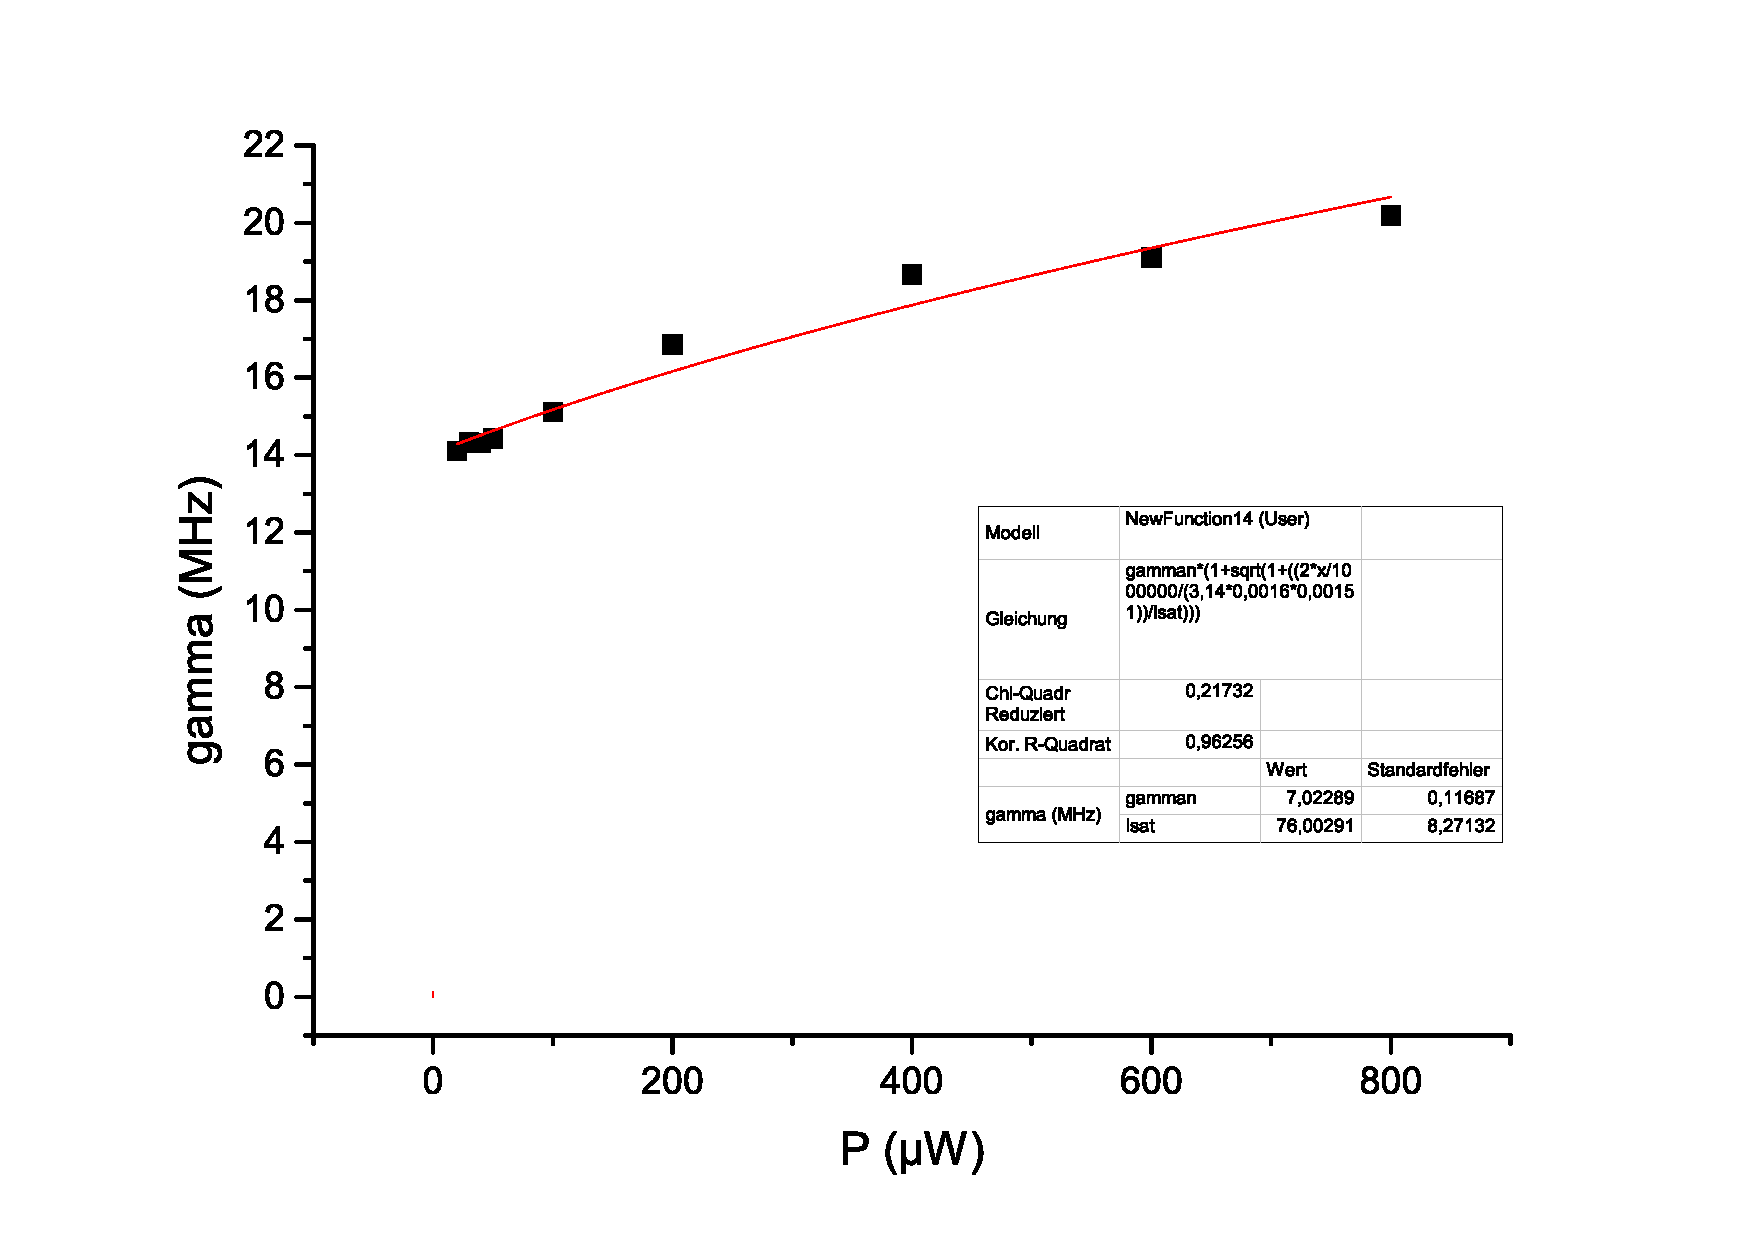
\includegraphics[width=1\textwidth]{./mitformelfit.pdf}
    \caption{Halbwertsbreiten $\Gamma$ der Lorentz-Resonanzen in Abh�ngigkeit der
			Pumpstrahlleistung $P$, Fit durch den theoretischen Verlauf
			nach \eqref{eq:mitformel}.}
\label{fig:mitformelfit}
\end{figure}
Wir erhalten:

\begin{equation}
	\begin{split}
	\gamma &= (7,02 \pm 0,12) \text{ MHz} \\
	I_{\text{sat}} &= (7,6 \pm 0,8) \frac{\text{mW}}{\text{cm}^2}
	\end{split} \nonumber
\end{equation}

\begin{figure}[!h]
  \subfigure[alle]{
  	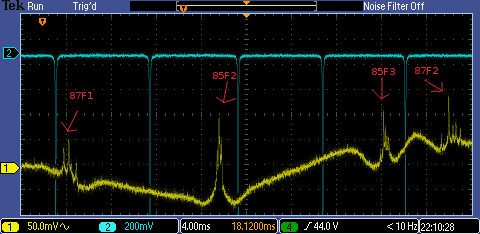
\includegraphics[width=1\textwidth]{./alle.png}
  } \\
  \subfigure[87F1]{
  	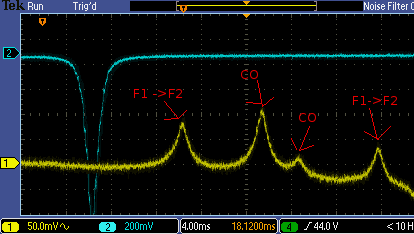
\includegraphics[width=0.5\textwidth]{./87F1.png}
  }
  \subfigure[85F2]{
  	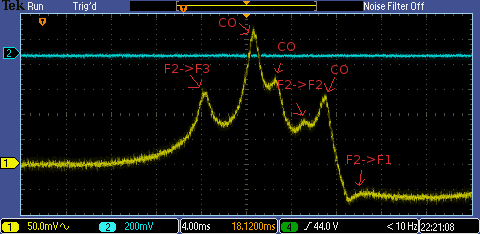
\includegraphics[width=0.5\textwidth]{./85F2.png}
  } \\
  \subfigure[85F3]{
  	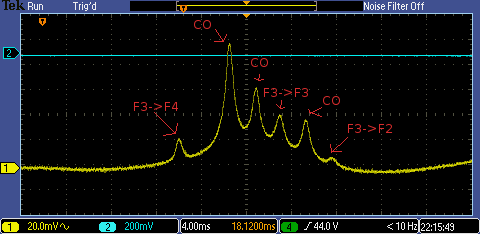
\includegraphics[width=0.5\textwidth]{./85F3.png}
  }
  \subfigure[87F2]{
  	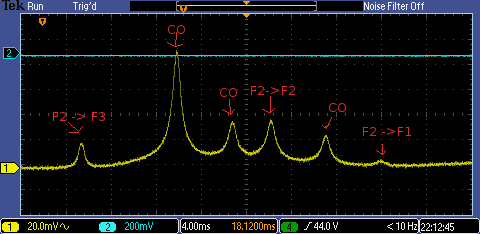
\includegraphics[width=0.5\textwidth]{./87F2.png}
  } \\
  \caption{Identifizierung der Hyperfeinstrukturlinien und der Crossover-Resonanzen}
\label{fig:identifi}
\end{figure}